%!TEX root = ../thesis.tex
%Adding the above line, with the name of your base .tex file (in this case "thesis.tex") will allow you to compile the whole thesis even when working inside one of the chapter tex files
%: ----------------------- introduction file header -----------------------
\chapter{Introduction} \label{chap:1}
\vspace{-1cm}
\textit{The chapter begins by outlining the motivation for studying winds from cool evolved stars, while simultaneously highlighting the problems associated with potential mass-loss mechanisms. The fundamental physics governing these winds along with their physical properties are then discussed. Their mass outflows are subsequently compared with other types of stars across the Hertzsprung Russel diagram and a description of how stars evolve to become red giants and red supergiants is also included. The second half of this chapter focuses on radio emission from stellar winds. The radio emission mechanisms that are relevant to this thesis are discussed and the terminology required to study cool evolved stellar winds at radio wavelengths is introduced. This chapter concludes with a brief outline of the remaining chapters within this thesis.}

\pagebreak

\section{Motivation for Researching Cool Evolved Stellar Winds}\label{sec:1.1}
Mass-loss from non-coronal spectral-type K through mid-M evolved stars plays a crucial role in galactic evolution and ultimately provides part of the material required for the next generation of stars and planets. This mass-loss occurs via a cool ($T_{e} \lesssim 10^4\,K$) wind with terminal velocities ($10 \lesssim v_{\infty} \lesssim 50$\,km\,s$^{-1}$), typically less than the photospheric escape velocity ($v_{\rm{esc}} \sim 100$\,km\,s$^{-1}$). The mass-loss rates for the red giants\footnote{The term \textit{red giant} excludes asymptotic giant branch stars throughout this thesis.} are significant, typically $10^{-11}-10^{-9}$\,$M_{\odot}$\,yr$^{-1}$, and are even higher for the more short-lived red supergiants (RSGs), typically $10^{-6}-10^{-4}$\,$M_{\odot}$\,yr$^{-1}$. This implies that a substantial fraction of the star's initial mass can be dispersed to the interstellar medium (ISM) during these post main sequence evolutionary stages \citep[e.g.,][]{schroder_2001}. Mass-loss from these stars is therefore a crucial factor governing stellar evolution \citep{chiosi_1986}, and also in explaining the frequency of supernovae in the galaxy \citep{van_loon_2010,dohm-palmer_2002}. Despite the importance of this phenomenon, and decades of study, the specific mechanisms that drive winds from evolved spectral-type K through mid-M stars remain unknown (clearly laid out by \citealt{holzer_1985} but still unsolved, e.g., \citealt{crowley_2009}). There is insufficient atomic, molecular, or dust opacity to drive a radiation-driven outflow \citep{zukerman_1995,jones_2008} and acoustic/pulsation models cannot drive the observed mass-loss rates \citep{sutmann_1995}. Ultraviolet (UV) and optical observations reveal an absence of significant hot wind plasma, and the winds are thus too cool to be Parker-type thermally-driven flows \cite[e.g.,][]{linsky_1979,haisch_1980,ayres_1981}. 

Magnetic fields are most likely involved in the mass-loss process, although current magnetic models are also unable to explain spectral diagnostics. High signal-to-noise ratio (S/N) \textit{Hubble Space Telescope} (\textit{HST}) UV spectra have revealed that the 1-D linear Alfv\'en wave-driven wind models of the 1980’s (e.g., \citealt{hartmann_1980,harper_1988}) are untenable \citep{harper_2001}. These models predict chromospheres as integral parts of a turbulent, extended, and heated wind acceleration zone, but the theoretical line profiles do not agree with the \textit{HST} spectra, \cite[e.g.,][]{judge_1998}. A new generation of theoretical models with outflows driven within diverging magnetic flux tubes have now emerged \citep{falceta_2006, suzuki_2007} but these too are not yet in agreement with observations \citep{crowley_2009}. Progress in this field continues to be driven by observations which can test existing models and theories, and provide new insights and constraints into the mass-loss problem.\\
\\
\textbf{The Advantages of Radio Observations}\\
Understanding the dynamics and thermodynamics of the atmospheres of late-type evolved stars will ultimately lead to a broader understanding of their mass-loss processes. Red supergiants have extended atmospheres which contain a mixture of atoms, ions, molecules, and dust, and are an ideal test bed for ideas and theories of mass-loss. These atmospheres are so extended that the closest red supergiants can be spatially resolved and imaged at centimeter and millimeter-wavelengths, both in continuum and molecular line emission. Such observations can yield direct measurements of the gas excitation temperature, velocity, and atmospheric structure, which can be used to provide essential constraints on the mass-loss process. 

The red giants on the other hand, have less extended atmospheres, which are dust free and contain only small abundances of molecules. They currently\footnote{ALMA and e-MERLIN will eventually be capable of spatially resolving the atmospheres of red giants.} cannot be spatially resolved at radio wavelengths, but their partially ionized outflows can still be detected at these wavelengths, providing an area-averaged sweep through the atmospheres of these stars. The lack of spatial resolution prevents the direct measurement of the fundamental atmospheric properties. However, point source radio observations can still be compared against existing atmospheric models based on shorter wavelength observations (e.g., models based on optical and UV observations). Such radio observations sample further out in the star's atmosphere than optical and UV observations and can test the validity of and improve upon existing model atmospheres. 

The research presented in this thesis attempts to understand the dynamics and thermodynamics of the atmospheres of red giants and RSGs, with the ultimate goal of gaining a deeper understanding of their mass-loss processes. To do so, we utilize the latest suite of radio interferometers which now have the capability of providing spatially resolved sensitive millimeter and centimeter observations of the atmsopheres of the closest RSGs, and sensitive multi-wavelength disk-averaged sweeps through the atmospheres of the closest red giants.

\section{On the Nature of Cool Evolved Stellar Atmospheres}\label{sec:1.2}
The study of stellar outflows from cool evolved stars began with the discovery of blue-shifted absorption features (i.e., ``P Cygni type'' profiles) in strong resonance lines from a number of bright red supergiants \citep{adams_1935}. They attributed these features to gradually expanding envelopes, even though the expansion speed velocity was small ($\sim 5$\,km\,s$^{-1}$) and much less than the photospheric escape velocity. \cite{spitzer_1939} analyzed similar data and devised a \textit{fountain model} for the atmospheres of red supergiants. In this model, radiation drives matter upwards from the photosphere until at some height, the ionization state of the matter changes, causing the radiation force to drop so that the matter falls back onto the star. Definitive evidence for mass-loss from cool evolved stars came from \cite{deutsch_1956} who observed a system which is now known to consist of an M5 giant (i.e., $\alpha$ Her), a G5 giant, and an unevolved medium F-type star \citep{reimers_1977}. He found that the same blue-shifted absorption features were present in the spectrum of both stars, which were not present in other single G5 giants. This indicated that both stars were enveloped in material which had been emitted from the M5 giant. The inferred expansion velocity at the distance of the G5 dwarf was sufficient to escape the system, thus confirming that matter was escaping the gravitational potential of the $\alpha$ Her system.

\begin{figure}[hbt!]
\centering 
          \includegraphics[trim=20pt 190pt 10pt 150pt,clip,width=15.0cm, height=12.0cm]{/home/eamon/thesis/thesis_template/1/dividing_line.ps}
\caption[The Linsky-Haisch dividing line]{A section of the H-R diagram showing the Linsky-Haisch dividing line which was proposed as a sharp division separating coronal (indicated by plus signs) from non-coronal (indicated by crosses) evolved late-type stars. Hybrid atmosphere stars are marked by circles. This image is taken from \cite{drake_1986} who carried out a 6\,cm survey of late-type evolved stars.}
\label{fig:1.2.1}
\end{figure}

Even though many later studies concluded that evolved late-type stars contained cool ($T_{e} < 1000$\,K) extended  circumstellar environments \citep[e.g.,][]{weymann_1962,gehrz_1971,bernat_1976,reimers_1975}, the physical properties of the ouflow between the photosphere and this cool outer environment remained unclear. An important discovery in late-type evolved stellar atmospheres resulted from the first ultraviolet survey of such stars using the \textit{International Ultraviolet Explorer} \citep[\textit{IUE};][]{macchetto_1978}. The survey revealed a ``transition region dividing line'' in the giant branch near spectral type K1 and in the supergiant branch near spectral type G5, which separates these stars based on the properties of their atmospheres \citep{linsky_1979, simon_1982}. In Figure \ref{fig:1.2.1} we show the approximate location of this dividing line in the H-R diagram. Stars blueward of the dividing line were found to possess chromospheres and transition regions like the Sun, while stars on the red side were found to possess chromospheres and cool winds. X-ray observations showed that this dividing line extended to coronal emission \citep{ayres_1981}. Around the same time, another class of late-type evolved star emerged which showed signs of possessing both a transition region and a cool wind \citep[e.g.,][]{reimers_1982}. Many of these so-called ``hybrid atmosphere'' stars now also show evidence for coronal emission, albeit much weaker than on the blue side of the dividing line \citep[e.g.,][]{ayres_1997}. 

\begin{figure}[hb!]
\centering 
\mbox{
          \includegraphics[trim=20pt 40pt 40pt 20pt,clip,width=7.5cm, height=11.0cm]{/home/eamon/thesis/thesis_template/1/wind_accel.ps} 
          \includegraphics[trim=25pt 40pt 10pt 20pt,clip,width=7.2cm, height=11.0cm]{/home/eamon/thesis/thesis_template/1/mg_ca_oplot.ps}
          }
\caption[\textit{HST }strong chromospheric lines]{\textit{Left:} \textit{HST} Goddard High-Resolution Spectrograph (GHRS) spectra showing the increase of wind scattering absorption velocity with optical depth for strong chromospheric lines. These data were taken for $\lambda$ Vel (a K5 Ib-II star) and show that it's wind accelerates in a quasi-steady manner. \textit{Right:} The \ion{Mg}{ii} \textit{h} and \textit{k} and \ion{Ca}{ii} H and K line profiles of $\alpha$ Boo. For many cool evolved stars, these strong resonant lines have often been compared to synthetic profiles to provide estimates of atmospheric properties. Three absorption components are present in the high S/N \textit{HST} data and originate from the ISM, the stellar wind, and an unknown source.}
\label{fig:1.2.2}
\end{figure}

The \textit{HST} allowed the important UV diagnostic transitions (e.g., lines from \ion{C}{ii}, \ion{Fe}{ii}, \ion{Mg}{ii}, and \ion{O}{ii}) to be observed with superb detail. The photon-scattering wind produces self-reversals in these chromospheric emission lines and have revealed that, for the most part, the red giant winds accelerate in a quasi-steady manner and are not the result of ballistic ejecta. This is inferred by the increase of wind scattering absorption velocity with optical depth, and thus height in the wind, as shown in Figure \ref{fig:1.2.2} for $\lambda$ Vel \citep{carpenter_1999}. The P Cygni-type line profiles, which are indicative of stellar outflows, are also shown in Figure \ref{fig:1.2.2} for the \ion{Mg}{ii} and \ion{Ca}{ii} resonance lines of $\alpha$ Boo (K2 III). For many evolved stars, these disk averaged emission line profiles have also provided crude estimates of atmospheric properties such as the mass-loss rate and terminal velocity, by comparing them to synthetic profiles based on detailed radiative transfer code \citep[e.g.,][]{robinson_1998}.

Chromospheres are the manifestation of surface convection and are found almost exclusively in the cool portion of the H-R diagram \citep{ayres_2010b}. These non-radiatively  heated regions of the inner atmosphere are present in the atmospheres of all late-type evolved stars. The isothermal pressure scale height, $H_{P}$, is the height in the atmosphere where the pressure drops by a factor of $e^{-1}$ and is given by
\begin{equation}
H_{P}=\frac{kT_e}{\mu m_{H} g} \propto \frac{T_{e}R_{\star}^2}{M_{\star}}.
\end{equation}
Here, $k$ is Boltzmann's constant, $T_{e}$ is the electron temperature, $R_{\star}$ is the stellar radius, $G$ is the gravitational constant, $M_{\star}$ is the stellar mass, $\mu$ is the mean mass per particle, and $m_{\rm{H}}$ is the mass of a hydrogen atom. The much larger radii of evolved stars means that their \textit{typical} scale height is over two orders of magnitude greater than that of the Sun. For example, a K5\,III star with a radius of $40\,R_{\star}$, will has a pressure scale height of $H_{P} \sim 0.005\,R_{\star}$. It is for this reason that their chromospheres are believed to be much more extended than the Sun's. The red supergiants are now known to have chromospheres which extend out to a few $R_{\star}$ \citep{lim_1998, harper_2001}. However, there is still much debate regarding the spatial extent of chromospheres in red giants. Recently, \cite{berio_2011} found that $\beta$ Ceti, a coronal giant, has a chromosphere which may extend out to $\sim 1.5\,R_{\star}$, while \cite{luttermoser_1994} found that the chromospheric spatial extend of an M6 giant to be $\le 1.05\,R_{\star}$. Determining the spatial extent of chromospheres in red giants is currently an area of active research.


\section{Basic Concepts of Stellar Winds}\label{sec:1.3}
The addition of energy above the photosphere is a requirement for a stellar outflow to escape the gravitational potential of a star. This energy input can be either in the form of a heat input (e.g., ambipolar diffusion heating),  a momentum input (e.g., radiation pressure on gas species), or as a combination of both. The momentum input is described by Newton's second law, $F=dp/dt$, where $F$ is the outward force and $p$ is the momentum. For this reason, the presence of an outward force is usually called momentum deposition, in contrast to energy deposition. The momentum deposition is governed by the momentum equation
\begin{equation}
F=\rho d\pmb{v}/dt
\end{equation}
where $\rho$ is the mass density, and $\pmb{v}$ is the velocity vector. In spherical symmetry, the velocity gradient is
\begin{equation}
\dfrac{dv(r,t)}{dt}=\dfrac{\partial v(r,t)}{\partial t}+\dfrac{\partial v(r,t)}{\partial r}\dfrac{dr(t)}{dt}=v\frac{dv}{dr},
\end{equation}
where we have assumed a stationary flow. The momentum equation for a flow being acted on by an outward directed force per unit mass, $f=f(r)$, is then
\begin{equation}\label{eq:moment}
v\frac{dv}{dr}=-\frac{1}{\rho}\frac{dP}{dr}-\frac{GM_{\star}}{r^2}+f
\end{equation}
where each of these terms have units of cm\,s$^{-2}$ \citep[e.g.,][]{lamers_1999}. The term on to the left of Equation \ref{eq:moment} is the acceleration, which is produced by the gas pressure gradient (first term on right), the gravity (second term on right), and some other force(s) which are contained in $f$. The gas pressure gradient term is directed outwards (positive) because $dP/dr < 0$. 
%The momentum equation was the cornerstone of the early attempts to explain the dynamics of the solar corona (See Section \ref{sec:1.4}).

The gas pressure gradient in Equation \ref{eq:moment} depends on the temperature structure of the outflow, which in turn depends on the heating and cooling. The effects of energy deposition can be expressed via the first law of thermodynamics 
\begin{equation}
\frac{du}{dt}=\frac{dq}{dt}-P\left(\frac{d\rho ^{-1}}{dt} \right)
\end{equation}
where $u=(3/2)(\mathcal{R}T/\mu)$ is the internal energy of the system per unit mass, $q$ is the net heat gained per unit mass, and the final term is the work done by the gas per unit time per unit mass. The time dependence can be removed using $d/dt=v\,d/dr$ to give
\begin{equation}\label{eq:1.6}
\frac{dq}{dr}=\frac{3}{2}\frac{\mathcal{R}}{\mu}\frac{dT}{dr}+P\frac{d\rho ^{-1}}{dr}.
\end{equation}
The ideal gas law can be written as 
\begin{equation}
\rho = \frac{\mu P}{\mathcal{R}T},
\end{equation}
and substituting this into the last term in Equation \ref{eq:1.6} gives the desired expression which relates the gas pressure to the heating:
\begin{equation}\label{eq:1.8}
\frac{1}{\rho}\dfrac{dP}{dr}=\dfrac{5}{2}\dfrac{\mathcal{R}}{\mu}\dfrac{dT}{dr}-\frac{dq}{dr}.
\end{equation}

The energy equation for stellar outflows can then be found by replacing the gas pressure term in the momentum equation with an expression which depends on the temperature structure of the outflow and the heating, i.e., combining Equations \ref{eq:moment} and \ref{eq:1.8}:
\begin{equation}\label{eq:1.9a}
\frac{d}{dr}\left(\frac{v^2}{2} + \frac{5\mathcal{R}T}{2\mu}-\frac{GM_{\star}}{r}\right)= f(r)+\frac{dq}{dr}.
\end{equation}
The combination of the terms inside the brackets on the left gives the total energy of the system per unit mass, with the first term being the kinetic energy of the flow, the second term being the enthalpy of the gas (the internal kinetic energy plus the capacity to do work), and the third term being the gravitational potential energy.  This equation tells us that the change in total energy of the gas as it moves a unit distance outwards from the star, is equal to the momentum input by the force and the heat input.

The energy equation in the form of Equation \ref{eq:1.9a} is called the \textit{Bernoulli} equation. Integrating the Bernoulli equation gives
\begin{align}\label{eq:1.10}
 e(r) &= \frac{v^2}{2} + \frac{5\mathcal{R}T}{2\mu}-\frac{GM_{\star}}{r} \nonumber \\
 & {} =e(r_{0}) + W(r) + q(r)
\end{align}
which states that the total energy per unit mass, $e(r)$, is equal to the initial energy, $e(r_{0})$, at the lower boundary $r_{0}$, plus the energy added to the wind in the form of the work done by the force, $W(r)$, and the heat deposition, $q(r)$. In other words, the total energy added to the wind per unit mass is used to increase the kinetic energy and the enthalpy of the wind, and to lift it out of the gravitational potential well. We can also compare the energy of the wind at the photosphere and at infinity, as described by \cite{lamers_1998}. At the photosphere, the total energy is negative and is just the gravitational potential energy, because $v_{\rm{esc}} \gg \mathcal{R}T_{\star}/\mu$ and  $v_{\rm{esc}} \gg v(R_{\star})$, i.e.,
\begin{equation}\label{eq:1.11a} 
e(r_{0}) \simeq -\frac{GM_{\star}}{R_{\star}}.
\end{equation}
At $r\rightarrow \infty$ the potential energy and the enthalpy both go to 0, and so the total energy is the kinetic energy,
\begin{equation}\label{eq:1.12a} 
e(r) \simeq \frac{v_{\infty ^2}}{2}.
\end{equation}
Substituting Equations \ref{eq:1.11a} and \ref{eq:1.12a} into Equation \ref{eq:1.10} then gives
\begin{equation}
\frac{v_{\infty ^2}}{2} \simeq -\frac{GM_{\star}}{R_{\star}} + W(r) + q(r).
\end{equation}
This equation tells us that a wind can only escape the gravitational potential of its star if there is an output force that provides sufficient momentum input or, if there is an energy source that provides sufficient heat input. These energy and momentum inputs are collectively known as wind driving mechanisms and in Section \ref{sec:1.4} we discuss the different mechanisms which occur across the H-R diagram.

\section{Stellar Wind Driving Mechanisms Across the H-R Diagram}\label{sec:1.4}
Stellar winds are a ubiquitous phenomenon across most of the H-R diagram. The various types of winds found throughout the H-R diagram can be broadly grouped into the three main categories of hot radiatively driven stellar winds, solar-type winds, and cool evolved stellar winds, as shown in Figure \ref{fig:1.2.3}. The cool evolved stellar winds can also be broadly grouped into the two categories of warm hybrid winds, and cool dense winds, as discussed in Section \ref{sec:1.2}. 

\begin{figure}[hbt!]
\centering 
          \includegraphics[trim=40pt 190pt 10pt 180pt,clip,width=15.0cm, height=11.0cm]{/home/eamon/thesis/thesis_template/1/cranmer.ps}
\caption[Stellar winds across the H-R diagram]{Stellar winds across the H-R diagram can be broadly grouped into the three main categories of hot radiatively driven stellar winds (upper left), solar-type winds (center right), and cool evolved stellar winds (upper right). The cool evolved stellar winds can also be broadly grouped into the two categories of warm hybrid winds (orange group) and non-coronal type (red group). \textit{Image credit:} Steven Cranmer.}
\label{fig:1.2.3}
\end{figure}

\subsection{Radiatively Driven Winds}\label{sec:1.4.1}
Stars earlier than spectral type $\sim$A2 emit their peak radiation in the UV, and so it was not until the early UV rocket observations that the presence of strong winds was confirmed from these stars \citep[e.g.,][]{morton_1967}. The broad P Cygni line profiles observed, indicated mass-loss rates as high as $10^{-5}\,M_{\odot}$\,yr$^{-1}$ and wind terminal velocities up to 3500\,km\,s$^{-1}$. Even though the lifetime of these massive hot stars is relatively short at just a few million years, their large mass-loss rates can substantially reduce the original stellar mass by a factor of two or more for the most massive \citep{owocki_2004}. Indeed, these stars typically end up as Wolf-Rayet (W-R) stars, which often appear to have completely lost their original envelope of hydrogen. These early-type stars do not exhibit the strong sub-surface convection that is present in solar and late-type stars (i.e., cool stars), and are therefore not believed to possess coronae. Their winds are therefore expected to remain at temperatures comparable to the star's surface, and so the gas-pressure term in Equation \ref{eq:moment} is not sufficient to drive their winds. Instead these stars are known to have a high radiative flux (since this scales as the fourth power of the surface temperature), and \cite{castor_1975} showed that this flux can accelerate a time-steady wind, by coupling with optically thick atomic lines in regions above the photosphere, where the continuum is optically thin. Therefore, the winds of these stars are effectively driven by the pressure of the star's emitted radiation and so the dominant term in Equation \ref{eq:moment} is a radiation pressure term contained within the parameter $f$.

\subsection{Solar Type Winds}\label{sec:1.4.2}
Our understanding of the wind driving mechanisms for stars with \textit{hot} solar-type winds is mainly based on solar theory and observations. Equation \ref{eq:moment} was the cornerstone of many early attempts to explain the dynamics of the solar corona. \cite{chapman_1957} assumed a static corona (i.e., the acceleration term was zero) and that the pressure gradient was the only outward force (i.e., $f=0$). Their results were unphysical, however, as they found that the density goes to infinity at large distances, and that the pressure was many orders of magnitude greater than that of the ISM. \cite{parker_1958} assumed that there was a continuous isothermal outflow of material from the Sun, caused only by the thermal pressure gradient term in Equation \ref{eq:moment} (i.e., $f=0$). He used the mass continuity equation, and the equation of state, to replace the pressure gradient term with a function depending only on velocity. Parker coined the solution to his simple analytical model as the ``solar wind'' and the predictions his model made for the solar velocity were confirmed shortly afterwards by some of the first space probes \citep[e.g.,][]{neugebauer_1962}. The assumptions of a radially expanding and isothermal outflow are not fully accurate in reality, however, and Parker's solution is an approximate characterization of the observed solar wind.

Coronal winds are generally tenuous, with mass-loss rates being too small to be of evolutionary importance. For example, at the Sun's current rate of mass-loss, about $10^{-14}\,M_{\odot}$\,yr$^{-1}$, its mass would be reduced by only $\sim 0.01 \%$ during its main sequence lifespan of $10^{10}$\,yr. Wind velocities are generally high ($200 \rightarrow 800$\,km\,s$^{-1}$), except for the very low gravity stars whose velocities are believed to be less \cite{drake_1986}. Although \cite{parker_1958} showed that the solar wind is a consequence of the thermal pressure gradient of the hot corona, the question of which mechanism drives the solar wind is still controversial, i.e., it is not understood how mechanical energy (convection) is transferred above the solar surface. The dissipation of Alf\'ven waves is a reliable candidate as a primary source of coronal heating \citep{cranmer_2011}, although other sources of energy and momentum probably exist \cite[e.g.,][]{parker_1983,parker_1988}. These waves can transfer energy from the surface convection up to the wind acceleration region because they can travel longer distances due to their incompressible nature \citep[e.g.,][]{hollweg_1973}. The dissipation of these waves then transfer momentum and energy to the gas via a cascade from large to small eddies \citep{verdini_2007}. Evolved stars blueward of the Linsky-Haisch dividing line also posses coronae and may share a similar mass-loss mechanism to that of coronal stars on the main sequence. 

\subsection{Cool Evolved Stellar Winds}\label{sec:1.4.3}
Cool evolved stars can generally be grouped into three main categories based on their mass and evolutionary status: (1) massive evolved red supergiants, (2) low and intermediate mass highly evolved stars ($0.8 - 8\,M\,_{\odot}$) known as asymptotic giant branch (AGB) stars, and (3) low and intermediate mass less evolved red giant stars. AGB stars lose a significant fraction of their mass through slow, massive winds at a rate of $10^{-8} \rightarrow 10^{-4}\,M_{\odot}$\,yr$^{-1}$ \citep{van_loon_2005}. This mass-loss occurs as a result of stellar pulsations \citep{habing_1996} which levitate material from the stellar surface, followed by the acceleration of dust grains by radiation pressure \citep{gehrz_1971}. 

The mass-loss mechanisms operating in red giants and red supergiants remain largely unknown and the theory governing mass-loss in AGB stars is not appropriate \citep{josselin_2007}. Red giants and red supergiants have small amplitude variations and so they do not pulsate in a similar manner to AGB stars. Also, significant amounts of dust are only found at large radii for red supergiants \citep{danchi_1994}, while red giants may have little or no dust in their outflows \citep{jones_2008}. One of the most plausible mass-loss mechanisms for these stars over the past few decades has been the transfer of energy and momentum to the wind by the dissipation of Alfv\'en waves. Unlike acoustic waves, Alfv\'en waves have large damping lengths that can transfer energy and momentum to the gas over many stellar radii. Alfv\'en wave models were originally known to result in high velocity winds, unlike what is observed for cool evolved stars. \cite{hartmann_1980} successfully showed that these observed low outflow velocities and high mass-loss rates could be reproduced if a wave damping mechanism is effective close ($r < 2\,R_{\star}$) to the star. \cite{hartmann_1984} constructed an Alfv\'en wave model for the red supergiant Betelgeuse which predicted its wind to have an electron temperature of 8000\,K at $4\,R_{\star}$ and remaining above 5000\,K out to $10\,R_{\star}$. However, the radio observations of \cite{lim_1998} revealed a much cooler wind cooler wind (see Chapter \ref{chap:3}) in conflict with the models of \cite{hartmann_1984}. One current school of thought is that giant convection cells may initiate the mass-loss process in red supergiants \cite[e.g.,][]{lim_1998}, although currently no model exits to explain how such a mechanism could operate.

\section{Red Giant and Red Supergiant Evolution}\label{sec:1.5}
Once a star has exhausted the hydrogen in its core, it evolves from the main sequence where its evolutionary future is dependent mainly by its mass. The vast majority of stars are of either low (i.e., $M_{\star} \lesssim 3\,M_{\odot}$) to intermediate mass (i.e., $ 3 \lesssim M_{\star} \lesssim 8\,M_{\odot}$), and evolve to become red giants, while the rare massive stars (i.e., $M_{\star} \gtrsim 8\,M_{\odot}$) generally evolve to become red supergiants. The stars studied in this thesis are either low mass or massive stars. These evolved late-type stars contain a condensed core with an extended envelope and have cooler effective temperatures than when on the main sequence. There is currently no consensus in the scientific community on why stars become red giants or red supergiants \citep[e.g.,][]{sugimoto_2000,stancliffe_2009}. A common explanation is that the initial expansion is driven by the envelope maintaining thermal equilibrium in response to increasing luminosity from the core. This expansion causes local cooling, allowing heavy elements to recombine, therefore causing an increase in opacity. This increase in opacity traps energy, leading to a runaway expansion that brings the star to the red giant or red supergiant region of the H-R diagram \citep{renzini_1992}. However, \cite{iben_1993} computed evolutionary models for intermediate mass stars with with the opacity held constant throughout, and showed that these models still became giants. This meant that opacity was not responsible for transition to a red giant, apparently in contradiction to \cite{renzini_1992}. 


\subsection{Change in Atmospheric Dynamics}\label{sec:1.5.1}
The expansion of a star's radius as it evolves off the main sequence greatly affects the dynamics of its atmosphere through the change of surface gravity. The decrease in surface gravity causes the density scale height to increase, resulting in very extended atmospheres. The mass-loss rate also increases due to the increase in the stellar surface area ($\propto R_{\star}^2$). In Table \ref{tab:1.1} we describe the typical properties of a 1 and $15\,M_{\odot}$ star both on the main sequence and as an evolved late-type star. We use these as examples to highlight the changes in the atmospheric dynamics when a star becomes a red giant or red supergiant. For these stars, the massive increase in stellar radius means that the density scale height, $H_{\rho}$, as a fraction of the stellar radius, $H_{\rho}/R_{\star} \propto T_{\mathrm{eff}}R_{\star}$, is $\sim 2$ orders of magnitude greater than when on the main sequence. There is also a drastic change in the terminal wind velocity, $v_{\infty}$. While on the main sequence, hot massive stars have wind velocities that are many times the photospheric escape velocity, $v_{\mathrm{esc}}$, while solar type stars have terminal wind speeds close to $v_{\mathrm{esc}}$. For evolved late-type stars the terminal wind velocity is generally much less than the photospheric escape velocity, signaling that the onset of these winds must be at several stellar radii. The final column in Table \ref{tab:1.1} is a comparison of the integrated mass-loss of these stars while on and off the main sequence. It is clear that during the time, $t$, spent in these evolved states, these stars lose a significant proportion of their initial mass, i.e., $\sim 30\%$ for massive stars and $\sim 10\%$ for the lower to intermediate mass stars. Such large quantities of mass-loss must have a significant impact on the evolution of the stars themselves and on their surrounding environments.


\begin{table}[!hbt]
\begin{center}
\caption[Properties of main sequence and evolved stars]
{Typical properties for main sequence and evolved 15 and $1\,M_{\odot}$ stars.}
\begin{tabular}{lccccccc}
\hline
\hline
\rule{0pt}{2.5ex}Evolutionary & $R_{\star}$ & $H_{\rho}/R_{\star}$ & $v_{\infty}$ & $v_{\mathrm{esc}}$ &$t$ & $\dot{M}_{\star}$& $t \times \dot{M}_{\star}$\\
 Stage$^{a}$ & ($R_{\odot}$) &  & (km\,s$^{-1}$) & (km\,s$^{-1}$) & (yr)$^{b}$  & ($M_{\odot}$\,yr$^{-1}$)& ($M_{\odot}$) \\
\hline
\rule{0pt}{2.5ex}MS O/B &5 &  $10^{-4}$ & 3000 & 1000&$10^{6}$ & $10^{-6}$&1\\
RSG & 1000 & $10^{-2}$& 20 & 75& $5\times10^{5}$&$10^{-5}$ &5\\ 
\hline
\rule{0pt}{2.5ex}MS F/G & 1 &$10^{-4}$ & 400& 600& $10^{10}$ &$10^{-14}$ &$10^{-4}$\\ 
RG & 40 & $10^{-2}$& 40& 100& $10^{9}$ & $10^{-10}$&0.1\\ 
\hline
\hline
\rule{0pt}{2.0ex}
\end{tabular}
\label{tab:1.1}
\begin{minipage}{19.5cm}
{\footnotesize \vspace{-0.4cm} $^{a}$ MS O/B = main sequence spectral type O and B stars. RSG = red supergiant. MS F/G= \\
main sequence spectral type F and G stars. RG = red giant.\\
\footnotesize  $^{b}$ The lifetimes for the evolutionary phases of the massive star are taken from \\ \cite{stothers_1969}}
\end{minipage}
\end{center}
\end{table}
\vspace{-0.5cm}

\subsection{Evolutionary Tracks}\label{sec:1.5.2}

Once a massive star on the main sequence has exhausted its  hydrogen core, it follows a nearly horizontal evolution across the H-R diagram where it usually becomes a helium burning RSG. Examples of these horizontal evolutionary tracks are shown in Figure \ref{fig:1.5.2.1} for masses between 9 and $120\,M_{\odot}$. Once the massive blue hydrogen burning stars move off the main sequence, they rapidly evolve across the ``yellow void'' passing through the very short-lived yellow supergiant stage \citep{levesque_2010}. As these stars evolve, the luminosity remains almost constant because massive stars do not develop degenerate cores and most of the mass is in radiative equilibrium. For stars with main sequence masses $\lesssim 25\,M_{\odot}$, like Betelgeuse, the RSG phase is the final stage before ending their lives as hydrogen-rich Type II supernovae. These stars lose a few $M_{\odot}$ during the RSG phase but do not lose enough to remove the whole H-rich envelope. Stars with masses $25\,M_{\odot}\lesssim M_{\star} \lesssim 40\,M_{\odot}$ lose their H-rich envelope during the RSG stage, turning the star into a W-R star. Finally, stars with $M_{\star} \gtrsim 40\,M_{\odot}$ never become RSGs, as their H-rich envelopes are blown off before the RSG stage can be reached.

\begin{figure}[hbt!]
\centering 
          \includegraphics[trim=10pt 250pt 0pt 200pt,clip,width=15.0cm, height=11.0cm]{/home/eamon/thesis/thesis_template/1/rsg_track2.ps}
\caption[Evolutionary tracks of massive stars]{Evolutionary tracks of massive stars from \cite{maeder_1987}. The shaded regions correspond to long-lived evolution phases on the main sequence, and during core He burning as a RSG (at log $T_{\mathrm{eff}} < 4.0$) or as a W-R star (at log $T_{\mathrm{eff}} > 4.8$).}
\label{fig:1.5.2.1}
\end{figure}

For low mass stars like Arcturus and Aldebaran, whose masses are between $\sim 1-2\,M_{\star}$ the post main sequence evolution can generally be categorized into four main stages as shown in Figure \ref{fig:1.5.2.2}. The following brief summary of these four stages is based on the conclusions of \cite{iben_1967} and \cite{ryan_2010}.

\begin{figure}[hbt!]
\centering 
    \includegraphics[trim=10pt 130pt 0pt 100pt,clip,width=12.0cm,height=11.0cm]{/home/eamon/thesis/thesis_template/1/solar_evol1.ps}
\caption[Evolution track of a low mass star]{Evolutionary track for $1\,M_{\star}$ star. The post main sequence evolution can generally be categorized into four main stages, i.e., the subgiant branch (SGB), the red giant branch (RGB), the red giant clump (RGC), and the asymptotic giant branch (AGB). Figure is adapted from \cite{ryan_2010}.}
\label{fig:1.5.2.2}
\end{figure}

\begin{enumerate}
%
\item The Subgiant Branch (SGB): This stage defines the period when a star has stopped core hydrogen burning but has not yet begun core helium burning. The core contracts therefore increasing the star's central temperature enough to initiate hydrogen fusion in a shell surrounding the core. The star swells and the effective temperature drops as it moves rapidly across the SGB, resulting in the Hertzsprung Gap.
%
\item The Redgiant Branch (RGB): As a star moves up the RGB its luminosity increases dramatically. The H-burning shell experiences a large gravitational force from the dense contracting core, causing the shell to compress and increase its energy output. A deep convective outer envelope penetrates the inner layers containing the remnants of H-burning resulting in newly synthesized nuclei being transported to the surface. This process is called the ``first dredge-up'' and the star's surface $^{12}$C/$^{13}$C ratio decreases due to the greater proportion of $^{13}$C in C/N-cycled material. At the tip of the RGB, the core finally reaches a sufficiently high temperature to cause helium burning, igniting the triple alpha process. The core begins to expand and the outer layers of the star contract, raising the surface temperature and leading to the output of less shell energy. This leads to a momentary decrease in luminosity and the star moves off the RGB.
%
\item The Redgiant Clump (RGC): Core helium burning and hydrogen shell burning characterize the RGC. A star's position on the RGC depends on its initial mass and composition, and  also on the amount of mass it has lost during the red giant phase. The pressure increases on the H-burning shell from the contracting envelope above, leading to an overall increase in luminosity. Core He-burning leads to an increasing molecular weight of the gas in the core, causing it to eventually contract. At the end of the RGC phase, all of the helium in the core is exhausted. The core collapses and the temperature rise ignites a shell of He-burning. The star now approaches the asymptotic giant branch.
%
\item The Asymptotic Giant Branch (AGB): The AGB is marked by a C-O core with two burning shells of He and H. The C-O core continues to grow and contract as the adjacent He shell burns. Stars with $M_{\star} \gtrsim 4\,M_{\odot}$ will undergo a ``second dredge up'', resulting again in the enhancement of the $^{12}$C/$^{13}$C ratio. With both shells burning, energy is consumed at an ever increasing pace and the star rapidly moves up the AGB while also developing periodic instabilities and generating large mass-loss rates. For stars with masses less than about $8\,M_{\odot}$, their cores never reach high enough temperatures to burn C-O and their evolution stops on the AGB. Higher mass stars can continue the process until iron is generated in the core and the evolution has gone as far as it can go.
\end{enumerate}
Traditionally, it has been almost impossible to distinguish between red giants burning helium in the core and those burning only hydrogen in an outer shell. Asteroseismology, is now becomming a powerful tool to help probe the internal structures of stars by using their natural oscillation frequencies \citep{beck_2011}, and has recently been used to distinguish between hydrogen and helium burning red giants \citep{bedding_2011}. In this thesis, the term ``red giant'' refers to evolved low mass stars which have not reached the AGB stage of evolution.

\section{Radio Emission from Stellar Atmospheres}\label{sec:1.6}
If we assume the Sun to be a nearly ideal blackbody with temperature $T=5800\,K$, then at 10\,GHz (i.e., 3\,cm), its flux density at Earth would be $\sim 10^{6}$\,Jy. However, at the distance of the nearest star other than the Sun (i.e., $\sim 1.3$\,pc), its flux density would be only $\sim 15\,\mu$\,Jy. Until recently\footnote{The new VLA has the ability to detect such values}, such a value would have been impossible to detect with even the most powerful radio telescopes. Nevertheless, stars have been detected at radio wavelengths for decades, which tells us immediately that such stars behave differently to the Sun at radio wavelengths. In fact, the discovery that such a huge range of stars emit detectable radio emission was one of the major and unexpected achievements of the old VLA \citep{white_2000}. A sample of the radio detected stars is plotted on a H-R diagram in Figure \ref{fig:1.6.1}, with the filled symbols representing the non-thermal emitters, and the open symbols representing the thermal emitters. 

\begin{figure}[ht!]
\centering 
          \includegraphics[trim=10pt 210pt 10pt 180pt,clip,width=15.0cm, height=11.0cm]{/home/eamon/thesis/thesis_template/1/radio_hr.ps}
\caption[Radio H-R diagram]{Sample of the radio detected stars plotted on a H-R diagram. The filled symbols represent non-thermal emitters while the open symbols represent the thermal emitters. The larger symbols are more radio luminous than the smaller symbols. In general, the sparse thermal emitters are stars with ionized or partially ionized extended stellar atmospheres whose radio emission comes from free-free interactions. Figure from \cite{white_2000}.}
\label{fig:1.6.1}
\end{figure}

It is clear that the majority of the main sequence and subgaint objects are non-thermal emitters. The only thermal emitters on the main sequence are the massive hot O-B stars which emit free-free radiation from their dense and ionized winds \cite[e.g.,][]{scuderi_1998}. Their radio spectrum are generally in good agreement with constant velocity isothermal stellar winds (i.e., $F_{\nu} \propto \nu ^{0.6}$ as discussed in Section \ref{sec:1.8.4}). These massive hot stars also emit non-thermal emission, which is believed to be produced by electron shock acceleration in the inhomogeneous wind. The cool region of the main sequence in Figure \ref{fig:1.6.1} contains red filled dots representing young F, G, K, and M dwarfs. These objects have ``non-thermal coronae'', which in addition to thermal populations of electrons at $10^{6-7}$\,K, contain non-thermal populations, which are trapped on closed magnetic field lines and produce strong radio emission. These objects are also flare stars, meaning that they occasionally emit strong radio outbursts. The blue filled circles near the center of the diagram are RS CVn binaries which consist of a late-type giant or subgiant and a close binary companion \citep{strassmeier_1993}. These systems generally rotate fast with typical orbital periods of a few days. Tidal forces between the close components have locked  their rotational periods to the orbital period. This fast rotational period in combination with outer convective zones generate intense magnetic activity and radio emission. 

Single (non-binary) cool evolved stars lack the characteristics which make the other stars, described above, radio bright. Even though they have outer convective zones, they rotate too slowly to generate, via an $\alpha - \Omega$ dynamo, the type of magnetic activity which make subgiant binaries and young cool dwarfs strong non-thermal radio emitters. They also lack the intense UV radiation field of the massive hot main sequence stars and their outflows are generally only partially ionized ($10^{-4} - 10^{-1}$). However, their large angular diameters coupled with their relatively large mass-loss rates, means that their partially ionized outflows can be detected at radio wavelengths. Red giants are feeble radio emitters however and up until the work presented in this thesis, only a small number have been detected at one or more radio wavelengths, and these have been modest S/N measurements. On the other hand, a few close-by red supergiants, like Betelgeuse, have mass-loss rates many orders of magnitude greater than the red giants and their partially ionized outflows can be easily detected at multiple radio wavelengths. These red supergiants also contain extended circumstellar envelopes (CSEs) which can be  sources of molecular line emission at radio wavelengths. 

\section{Radio Emission Mechanisms}\label{sec:1.7}
The two radio emission mechanisms which are most relevant in this thesis are thermal Bremsstrahlung/free-free emission, and molecular line emission. Both of these emission mechanisms produce incoherent radiation and are discussed in the following sections. Under certain plasma conditions, coherent radiation can be produced due to resonances between particles and characteristic electromagnetic waves.  This results in electron energy being converted into some natural wave mode of the plasma, such as Langmuir waves (plasma oscillation) or electron-cyclotron waves. The main characteristic frequencies of a plasma are the electron plasma frequency
\begin{equation}
\nu _{p} = \frac{\omega _{p}}{2\pi}=\left( \frac{n_e e^2}{\pi m_e}\right)^{1/2} \approx 9000 n_e ^{1/2}\ \ \ \ \rm{Hz}
\end{equation}
and the electron-cyclotron frequency
\begin{equation}
\nu _{B}= \frac{\Omega _{B}}{2\pi}=\frac{eB}{2\pi m_e c} \approx 2.8B\ \ \ \ \rm{MHz}
\end{equation}
where $n_e$ is the electron number density with units $\rm{cm}^{-3}$, and $B$ is the magnetic field strength with units G\footnote{1 Gauss (G)\,$= 1\times 10^{-4}$ tesla (T).}. 

\subsection{Thermal Free-free (Bremsstrahlung) Emission}\label{sec:1.7.1}
Thermal Bremsstrahlung from an ionized or partially ionized plasma is often called free-free emission because it is produced by free electrons which are deflected off ions without being captured. For free-free radio emission, the distant Coulomb interactions of electrons with ions, which cause small angle deflections, are much more important than the rare close encounters and large deflections \citep{dulk_1985}. The free-free emission, which is the energy radiated per unit volume, per unit time, per unit frequency, is given in \cite{rybicki_1979} as:
\begin{equation}\label{eq:1.7.1}
\varepsilon _{\nu} ^{ff} = 6.8 \times 10^{-38}Z^{2}n_{e}n_{i}T^{-1/2}e^{-h\nu /kT}g_{ff}\ \ \ \ \rm{erg}\,\rm{cm}^{-3}\,s^{-1}\,\rm{Hz}^{-1}
\end{equation}
Here, $g_{ff}$ is the free-free Gaunt factor and is a correction factor which is a function of electron energy and frequency of emission. Extensive tables and graphs of $g_{ff}$ exist in the literature \citep[e.g.,][]{karzas_1961}. The free-free emissivity, which is a fundamental term in the equation of radiative transfer is then
\begin{equation}\label{eq:1.7.2a}
j_{\nu} ^{ff}=\frac{\varepsilon _{\nu} ^{ff}}{4\pi}.
\end{equation}
The free-free radio opacity can then be found from Kirchoff's law and is discussed in Section \ref{sec:1.8.3}.

\subsection{Molecular Line Emission}\label{sec:1.7.2}
A diatomic molecule such as CO or SiO, can vibrate (stretch) along the internuclear axis and can also undergo rotational motion around an axis perpendicular to the internuclear axis. The rotational levels of these molecules are designated by a single vibrational quantum number, $v$, and a rotational quantum number, $J$. Most of the diatomic molecular lines observed in the radio spectrum are from the rotational levels. These rotational energy levels are approximately those allowed by quantum mechanics for a rigid rotator, i.e., a linear molecule that does not change shape as it rotates. The rotational kinetic energy is
\begin{equation}\label{eq:1.7.2}
E_{\mathrm{rot}} = \frac{I\omega ^2}{2}
\end{equation}
where $I = m_{r}r_{0}^2$ is the moment of inertia, $m_{r}$ is the reduced mass, $r_{0}$ is the separation of the two masses, and $\omega$ is the angular velocity of the rotation. The quantization of angular momentum, $L$, to integer multiples of $\hbar$ leads to $L=J\hbar$, where $J=1,2,\dots$. Equation \ref{eq:1.7.2} can then be written as
\begin{equation}
E_{\mathrm{rot}}(v,J) = \frac{L^2}{2I}=\frac{J(J+1)\hbar ^2}{2I}=\frac{J(J+1)\hbar ^2}{2m_{r}r_0 ^2}=B_{v}J(J+1)
\end{equation}
where $B_{v}$ is the \textit{rotation constant} and is subscripted $v$ because the moment of inertia depends on the vibrational state. $^{12}$C$^{16}$O and $^{28}$Si$^{16}$O, two molecules studied in this thesis, have rotation constant values of $B_{v}=2.766$ and 1.042\,K, respectively \cite{huber_1979}.

\begin{figure}[hb!]
\centering 
\mbox{
          \includegraphics[trim=80pt 60pt 40pt 60pt,clip,width=4.5cm, height=10.0cm]{/home/eamon/thesis/thesis_template/1/ladder.ps}
          \includegraphics[trim=0pt 0pt 0pt 20pt,clip,angle=90,width=10.5cm, height=10.0cm]{/home/eamon/thesis/thesis_template/1/rotational_levels.ps}
          }
\caption[Molecular ladder plot and relative populations]{\textit{Left:} The radio spectrum of $^{12}$C$^{16}$O resembles a \textit{ladder} with each step being a harmonic of the fundamental frequency that is determined solely by the moment of inertia. This molecule has a relatively small moment of inertia and therefore has no cm-wavelength lines. \textit{Right:} The relative populations of the rotational levels of $^{12}$C$^{16}$O and $^{28}$Si$^{16}$O at temperatures of 70 and 200\,K, the excitation temperatures \cite{bernat_1979} derived for the two circumstellar outflows of Betelgeuse. At lower temperatures, the distribution of the relative populations of the rotational levels is towards lower $J$s and is shifted towards higher $J$s at higher temperatures.}
\label{fig:1.7.2}
\end{figure}

Pure rotational transitions, $J\rightarrow J-1$, have energy $h\nu = 2B_{v}J$. It is straightforward to show that the rotational transitions $J=1-0$ and $J=2-1$ of the CO molecule results in spectral lines at frequency 115.2712 and 230.5424\,GHz. A radio spectrum of a particular molecular species will resemble a \textit{ladder} as shown in Figure \ref{fig:1.7.2}. Each step in the plot are all harmonics of the fundamental frequency that is determined solely by the moment of inertia of that species. As $\nu \propto m^{-1}r_{0}^{-2}$, large heavy molecules in CSEs may be seen at centimeter wavelengths, but smaller and lighter molecules such as CO and SiO emit only at millimeter wavelengths. 
Rotational states are usually populated according to Boltzmann's law at densities and temperatures where vibrational levels cannot be excited. In this case the Boltzmann equation can be used to find the relative populations of the levels:
\begin{equation}
\frac{n_{J}}{n_{0}}=(2J+1)e^{-B_{v}J(J+1)/T}.
\end{equation}
The partition function, $Z(T)$, is found by summing over all levels, $i$,
\begin{eqnarray}
Z(T) & = & \sum\limits_{i}^{\infty}g_{i}e^{-E_{i}/kT} \\
             & = & \sum\limits_{J=0}^{\infty}(2J+1)e^{-B_{v}J(J+1)/T} \\
              & \approx & \int ^{\infty} _{0}(2J+1)e^{-B_{v}J(J+1)/T} dJ =T/B_{v}.
\end{eqnarray}
where we have replaced the sum over discrete values of $J$ with a continuous integral \citep{shu_1991}. The relative rotational populations within a given vibrational state are then
\begin{equation}\label{eq:1.24a}
\dfrac{n_{J}(v)}{n(v)} \approx \frac{(2J+1)B_{v}}{kT}e^{-B_{v}J(J+1)/T}.
\end{equation}
This distribution is plotted in Figure \ref{fig:1.7.2} for the ground vibrational levels of CO and SiO and shows how the levels are populated with respect to one another at two different temperatures\footnote{These are the expected excitation temperatures of the two CSE flows of Betelgeuse.}. The distribution is such that at low temperatures, the rotational levels are more relatively populated at lower $J$s, while higher $J$s become relatively more populated at higher temperatures. Differentiating Equation \ref{eq:1.24a} with respect to $J$
gives the most probable occupied rotational state, $J_{\rm{mp}}$, as a function of temperature,
\begin{equation}
J_{\mathrm{mp}}=\sqrt{\frac{T}{2B_{v}}}-\frac{1}{2}.
\end{equation}
The total flux produced by a transition out of the most probable occupied state, $J_{\mathrm{mp}}, J_{\mathrm{mp}}-1$, will not necessarily be the transition that emits the most flux. This is because the total flux produced by any rotational transition is
\begin{equation}
F_{J,J-1}=\Delta E_{J,J-1}n_{J}A_{{J,J-1}}
\end{equation}
where the spontaneous emission coefficient can be written as
\begin{equation}
A_{J,J-1} =2.14\times 10^{-7}\frac{J^4}{2J+1} \ \ \ \rm{s}^{-1}
\end{equation}
\citep{draine_2011}, and $\Delta E_{J,J-1}=2B_{v}J$. Therefore, the total flux not only depends on the population of the level but also on the change in energy and the probability of undergoing that transition.

\section{Radio Observations of Stellar Atmospheres}\label{sec:1.8}
In the following sections we present the basic definitions used to describe radio observations of stellar atmospheres. We define the \textit{brightness temperature} which is commonly used in radio astronomy to measure the brightness of a source, along with its relationship to the fundamental quantity measured by a radio telescope, the \textit{flux density}. Focusing on thermal emission, we describe how the flux density varies with frequency when observing both optically thin and optically thick stellar atmospheres, and conclude by discussing how molecular emission line profiles can be studied at radio wavelengths.

%At this point it is well to draw the distinction between blackbody radiation, where I, = B,, and thermal radiation, where S,, = B,. Thermal radiation becomes blackbody radiation only for optically thick media
\subsection{Brightness Temperature}\label{sec:1.8.1}
In thermodynamic equilibrium the spectral distribution or brightness, $B_{\nu}$, of the radiation of a black body with temperature $T_{e}$ is given by the Planck law
\begin{equation}\label{eq:1.1}
B_{\nu}(T_{e})=\frac{2h\nu ^3}{c^2}\frac{1}{e^{h\nu /kT_{e}}-1}
\end{equation}
and has units of erg\,s$^{-1}$\,cm$^{-1}$\,Hz$^{-1}$\,sr$^{-1}$. One can easily switch to a wavelength form using  $B_{\nu}d\nu = B_{\lambda}d\lambda$. When $h\nu /kT_{e} \ll 1$ Equation \ref{eq:1.1} becomes the \textit{Rayleigh-Jeans Law}
\begin{equation}
\label{eq:1.2}
B_{\nu}(T_{e})=I_{\nu}(T_{e})=\dfrac{2\nu ^2kT_{e}}{c^2}.
\end{equation}
This equation does not contain Plank's constant and therefore is the classical limit of the Planck Law. We have also included the specific intensity, $I_{\nu}$, in Equation \ref{eq:1.2} as it has the same units as the spectral brightness and for blackbody radiation, $I_{\nu}(T_{e}) = B_{\nu}(T_{e})$. This equation is valid for all thermal radio sources except in the millimeter or sub-millimeter regime at low temperatures \citep{rohlfs_1996}. In the Rayleigh-Jeans relation, the brightness is strictly proportional to the thermodynamic temperature of the black body. In radio astronomy it is customary to measure the brightness of an object by its \textit{brightness temperature}, $T_{\rm{b}}$. Therefore, the brightness temperature is the temperature at which a blackbody would have to be in order to reproduce the observed brightness of an object at frequency $\nu$ and is defined as
\begin{equation}\label{eq:1.3}
T_{\rm{b}}\equiv \frac{c^2}{2k\nu ^2}I_{\nu}. 
\end{equation}
If $h\nu /kT \ll 1$ and if $I_{\nu}$ is emitted by a blackbody, then $T_{\rm{b}}$ is the thermodynamic temperature of the source. If other processes are responsible for the emission or if the frequency is so high that Equation \ref{eq:1.2} is not valid, then $T_{\rm{b}}$ is different from the thermodynamic temperature of a black body.

The equation of radiative transfer describes the change in specific intensity of a ray along the line of sight in a slab of material of thickness $ds$
\begin{equation}\label{eq:1.4}
\frac{dI_{\nu}}{ds}=j_{\nu} - \kappa _{\nu}I_{\nu},
\end{equation}
where $j_{\nu}$ and $\kappa _{\nu}$ are the emissivity (in erg\,s$^{-1}$\,cm$^{-3}$\,Hz$^{-1}$\,sr$^{-1}$) and the absorption/opacity coefficient (in cm$^{-1}$) of the plasma. In thermodynamic equilibrium the radiation is in complete equilibrium with its surroundings and the brightness distribution is described by the Planck function
\begin{equation}\label{eq:1.5}
\dfrac{dI_{\nu}}{ds}=0, \ \ \ \ \ \ I_{\nu}= \frac{j_{\nu}}{\kappa _{\nu}}=B_{\nu}(T_e).
%=\frac{c^2}{2k\nu ^2}T_{e}.
\end{equation}
Equation \ref{eq:1.4} can be solved by first defining the optical depth, $d\tau _{\nu}$, as
\begin{equation}
d\tau _{\nu}=-\kappa _{\nu}ds,
\end{equation}
and then integrated by parts between 0 to $s$, and $\tau$ to 0, to give 
\begin{equation}
I(s) = I(0)e^{-\tau(s)} + \int ^0 _{\tau (s)}e^{-\tau} \frac{j_{\nu}}{\kappa _{\nu}}d\tau.
\end{equation}
The second term within the integral is known as the source function, $S_{\nu}$, and this can be taken outside of the integral in the case of a homogeneous source, i.e., one for which both the emissivity and absorption coefficient are constant along the ray path. The solution then to the equation of radiative transfer for a homogeneous source is
\begin{equation}\label{eq:1.9}
I_{\nu} = I_{0}e^{-\tau} + \frac{j_{\nu}}{\kappa _{\nu}}(1 - e^{-\tau}).
\end{equation}
Using Equations \ref{eq:1.3} and \ref{eq:1.5} one obtains
\begin{equation}
T_{b} = T_{0}e^{-\tau} + T_{e}(1 - e^{-\tau}).
\end{equation}
This equation assumes thermodynamic equilibrium and so only holds for a thermal source. If $T_{e}$ is replaced with $T_{\rm{n-t}} = h\nu/k$  then this equation becomes valid for a homogeneous non-thermal source, i.e.,
\begin{equation}
T_{b} = T_{0}e^{-\tau} + T_{\rm{n-t}}(1 - e^{-\tau}).
\end{equation}
For an isolated thermal source, there are two limiting cases:
\begin{equation}\label{eq:1.11}
T_{b} = T_{e} \ \ \ \ \mathrm{(i.e.,\ for\ optically\ thick}\ \tau \gg 1)
\end{equation}
and
\begin{equation}\label{eq:1.12}
T_{b} = \tau T_{e} \ \ \ \ \mathrm{(i.e.,\ for\ optically\ thin}\ \tau \ll 1).
\end{equation}
In Equations \ref{eq:1.11} and \ref{eq:1.12}, $T_{e}$ can also be replaced by $T_{\rm{n-t}}$ if the radio emission is non-thermal. Also, these equations are only valid if the source is spatially resolved. If the source is unresolved then a lower limit to $T_{e}$ or $T_{\rm{n-t}}$ is found.

\subsection{Brightness Temperature and Flux Density}\label{sec:1.8.2}
The flux density, $F_{\nu}$, is a fundamental quantity measured by a radio telescope and is usually measured in Janskys (Jy) where 1\,Jy$ = 1\times 10^{-26}$\,W\,m$^{-2}$\,Hz$^{-1}$. The observed flux density measured by the radio telescope is related to the specific intensity by
\begin{equation}\label{eq:1.13}
F_{\nu} = \int _{\Omega} I_{\nu}\,d\Omega
\end{equation}
%($\Omega \approx \pi R_{\star}^2/d^2$)
where $\Omega$ is the solid angle subtended by the source or the antenna beam. The radio emission from evolved cool stars is almost purely thermal and so Equation \ref{eq:1.13} becomes 
\begin{equation}
F_{\nu} =  \frac{\pi R_{\star}^2}{d^2}\frac{2k\nu ^2T_{b}}{c^2}.
\end{equation}
The angular diameter of a star in radians is $\phi _{\star}=2R_{\star}/d$ and so
\begin{equation}
F_{\nu}=\frac{\pi k\phi _{\star}^2 T_b}{2\lambda ^2}.
\end{equation}
If $\phi _{\star}$ has major and minor axes $\phi _{\rm{maj}}$ and $\phi _{\rm{min}}$ then
\begin{equation}
T_{b} (K)=1.96F_{\nu}(\mathrm{mJy})\left(\frac{\lambda}{\mathrm{cm}}\right)^2\left(\frac{\phi _{\mathrm{min}}}{\mathrm{arcsec}} \frac{\phi _{\mathrm{min}}}{\mathrm{arcsec}}\right)^{-1}.
\end{equation}
Therefore, if an optically thick stellar atmosphere can be spatially resolved at long wavelengths (i.e., $\phi _{\rm{maj}}$ and $\phi _{\rm{min}}$ can be measured) then the flux density at a particular wavelength gives the brightness temperature and therefore the electron temperature. Unfortunately, the number of stars that can have their atmospheres spatially resolved at radio wavelengths is low due to their relatively small angular diameters. As an example, Betelgeuse has the largest angular diameter of any star other than the Sun in the northern hemisphere, but at 6\,cm (i.e., 6\,GHz) its atmosphere is barely resolvable with the VLA in its most extended configuration, which provides a spatial resolution of $\sim 330$\,mas. However, different layers of stellar atmospheres can still be probed, even if the radio emission is unresolved, due to the nature of the free-free radio opacity which is discussed in the next section.

\subsection{Thermal Free-free Radio Opacity}\label{sec:1.8.3}
In Section \ref{sec:1.7.1} we gave an expression for the thermal free-free emissivity of an ionized gas. Kirchoff's law can be used to find the thermal radio free-free opacity (absorption coefficient):
\begin{equation}
\frac{j_{\nu}^{ff}}{\kappa _{\nu}^{ff}}=\frac{2h\nu ^3}{c^2}\frac{1}{e^{h\nu /kT}-1}
\end{equation}
Using Equation \ref{eq:1.7.1} and \ref{eq:1.7.2a} then provides a value for the free-free radio opacity which is corrected for stimulated emission:
\begin{equation}
\kappa _{\nu}^{ff} = \frac{0.018Z^2n_{e}n_{i}g_{ff}(\nu ,T_{e})}{T_{e}^{1.5}\nu ^{2}}\ \ \ \ \rm{cm^{-1}}.
\end{equation}
The Gaunt factor is slightly dependent on temperature and frequency and at cm-wavelengths is given by
\begin{equation}
g_{ff}^{cm}=11.96T_{e}^{0.15}\nu ^{-0.1}
\end{equation}
\citep{Altenhoff_1960}, while in the  sub-millimeter regime it is slightly different
\begin{equation}
g_{ff}^{sub-mm}=24.10T_{e}^{0.26}\nu ^{-0.17}
\end{equation}
\citep{harper_2013,hummer_1988}. The abundant species in the atmospheres of cool evolved stars are either neutral or single ionized so that $Z=1$ and $n_{e} = n_{i}$. Focusing on centimeter wavelengths, the radio opacity is then
\begin{equation}\label{eq:1.22}
\kappa _{\nu}^{ff} = \frac{0.212n_{e}^2}{T_{e}^{1.35}\nu ^{2.1}}\ \ \ \ \ \ \rm{cm}^{-1}.
\end{equation}
Therefore, the free-free opacity increases towards lower frequencies as $\kappa _{\nu}^{ff} \propto \nu ^{-2.1}$ (or longer wavelengths as $\kappa _{\lambda}^{ff} \propto \lambda ^{2.1}$). This means that the optical depth, $\tau _{\lambda}= \int \kappa _{\lambda} dr$, also increases towards longer wavelengths implying that the effective radius (i.e., the radius where $\tau _{\lambda} = \tau _{\rm{radial}}$) will increase with longer wavelengths. As a result, different layers of unresolved stellar atmospheres can be probed by observing them at different radio wavelengths.

\begin{figure}[ht!]
\centering 
          \includegraphics[trim=10pt 160pt 10pt 140pt,clip,width=13.0cm, height=11.0cm]{/home/eamon/thesis/thesis_template/1/radio_opacity.ps}
\caption[\ion{H}{ii} region radio spectrum]{The radio spectrum for a hypothetical \ion{H}{ii} region with no background illuminating source. At long wavelengths the source becomes opaque and has a black body like spectrum with $\alpha = 2$. At short wavelengths where $\tau _{\nu} \ll 1$, the \ion{H}{ii} region is almost transparent and $\alpha = -0.1$. Image adapted from NRAO's \textit{Essential Radio Astronomy} course.}
\label{fig:1.5.3}
\end{figure}

For thermal radiation, the solution to the equation of radiative transfer (i.e, Equation \ref{eq:1.9}) for a plasma with no background source can be written as 
\begin{equation}\label{eq:1.23}
I_{\nu} = B_{\nu}(1-e^{-\tau}).
\end{equation}
An example of such a source is an isolated \ion{H}{ii} region. At long enough wavelengths the \ion{H}{ii} region becomes opaque so that $\tau _{\nu} \gg 1$. Equation \ref{eq:1.23} then tells us that the spectrum approaches that of a black body with a flux density varying as $F_{\nu} \propto \nu ^{2}$. At short wavelengths where $\tau _{\nu} \ll 1$, the \ion{H}{ii} region is almost transparent, and the flux density becomes
\begin{equation}
F_{\nu} \propto \frac{2kT_{e}\nu ^2}{c^2}\tau _{\nu} \propto \nu ^{-0.1}.
\end{equation}
These two scenarios are shown in Figure \ref{fig:1.5.3} along with the point where these two slopes intersect which corresponds to the frequency at which $\tau \simeq 1$. When the radio spectrum is plotted on a log-log plot as in Figure \ref{fig:1.5.3}, the spectral slope is referred to as the spectral index, $\alpha$, and is defined:
\begin{equation}
\alpha = \frac{d\,\mathrm{log}\,F_{\nu}}{d\,\mathrm{log}\,\nu}.
\end{equation}
The relatively nearby $\alpha$ Sco binary system ($d=185\pm 60$\,pc; \citealt{perryman_1997}), which consists of a M1.5\,Iab red supergiant and a B2.5\,V star was observed by \cite{hjellming_1983} with the old VLA. They found that the massive wind of the red supergiant is ionized around the B2.5\,V star creating a H\,II region. The emission from the H II region had a spectral index of $\alpha = 0.1$, consistent with optically thin emission. The radio excess from the red supergiant was $\alpha = 1.05$, intermediate between that of an isothermal stellar disk emission (i.e., $\alpha = 2$), and an isothermal, constant velocity and ionization fraction wind whose spectral index is discussed in the following section.



\subsection{Radio Excess from Stellar Winds}\label{sec:1.8.4}
Most cool evolved stars have partially ionized outflows which emit an excess of continuum emission at long wavelengths. This flux excess is due to thermal free-free emission and is measured relative to the expected photospheric radio flux. If the atmosphere only consisted of a static homogeneous isothermal chromosphere then the radio spectrum would be the summation of the Rayleigh-Jeans tail of the Planck function from the photosphere and the \ion{H}{ii} spectrum discussed in the previous section. At long wavelengths then, this spectrum would again have a power law of slope $F_{\nu} \propto \nu ^{2}$. Cool evolved stellar atmospheres cannot in general be described by this simple model because they possess stellar winds which are escaping the gravitational potential of the star. The atmospheric density thus varies with distance from the star. In this section we briefly outline a simple analytical model for the centimeter radio flux for a star with an isothermal, constant velocity and ionization fraction wind. In Chapter \ref{chap:6} we relax some of these assumptions about the atmosphere's properties to derive a more complete description of the centimeter radio spectrum for these stars.

\begin{figure}[hbt!]\label{fig:1.5.4}
\centering 
          \includegraphics[trim=10pt 310pt 10pt 280pt,clip,width=15.0cm, height=7.0cm]{/home/eamon/thesis/thesis_template/1/radio_spec.ps}
\caption[Schematic for stellar wind radio emission excess]{In spherical geometry the observer integrates along a ray path in the $z$ direction, with impact parameter $b$, to calculate the total optical depth $\tau _{\nu}$, at a frequency $\nu$.}
\label{fig:1.5.4}
\end{figure}

To calculate the optical depth, we assume spherical geometry and integrate along a ray in the $z$ direction with impact parameter $b$, as shown in Figure \ref{fig:1.5.4}. The total optical depth at a frequency $\nu$ is then
\begin{equation}
\tau _{\nu} = \int ^{\infty} _{-\infty} \kappa _{\nu} dz
\end{equation}
where the opacity is defined in Equation \ref{eq:1.22}. For a constant velocity the electron density is just $n_{e}(r)=n_{e}(r_{0})^2(r_{0}/r)^2$ and so the optical depth can be written as
\begin{equation}
\tau _{\nu} = \frac{0.212n_{e}(r_{0})^2r_{0}^4}{T^{1.35}\nu ^{2.1}}\int ^{\infty} _{\infty}\frac{dz}{(b^2 + z^2)^2}.
\end{equation}
The solution to this integral is given by
\begin{equation}
\int ^{\infty} _{-\infty} \frac{dz}{(b^2 + z^2)^{A/2}}=b^{1-A}\sqrt{\pi}\frac{\Gamma (A/2 -1/2)}{\Gamma (A/2)}
\end{equation}
and so the total optical depth along a ray with impact parameter $b$ is:
\begin{equation}
\tau _{\nu} = \frac{C}{b^3}\ \ \ \ \ \ \mathrm{where}\ \ \ C=\frac{0.333n_{e}(r_{0})^2r_{0}^4}{T^{1.35}\nu ^{2.1}}.
\end{equation}

To calculate the flux density we use Equation \ref{eq:1.13} and assume that the source function is given by the Planck function in the Rayleigh-Jeans approximation:
\begin{equation}
F_{\nu} = \frac{2\pi}{d^2}\frac{2\nu ^2 kT}{c^2} \int ^{\infty} _{0}(1-e^{-C/b^3})bdb.
\end{equation}
This integral can be solved using the following expression
\begin{equation}
\int ^{\infty} _{0}y^{v-1}(1-e^{-uy^p})dy=\frac{-1}{|p|}u^{-v/p}\Gamma \left(\frac{v}{p} \right),
\end{equation}
which is given in \cite{gradshteyn_1994}. The solution to our integral is then $1.3395C^{2/3}$ and so the total flux density can be written as 
\begin{equation}\label{eq:1.32}
F_{\nu} = 2.574\frac{\pi k}{c^2}\dfrac{n_e(r_0)^{4/3}r_0^{8/3}T^{0.1}\nu ^{0.6}}{d^2}.
\end{equation}
Substituting in the mass continuity equation gives
\begin{equation}\label{eq:1.33}
F_{\nu} = 0.277\frac{k}{c^2 m_{\mathrm{H}}^{4/3}}\dfrac{\dot{M}^{4/3}T^{0.1}\nu ^{0.6}}{\mu ^{4/3}v^{4/3}d^2}.
\end{equation}
where $\mu$ is the mean atomic weight of the gas and $m_{\rm{H}}$ is the mass of a hydrogen atom. This equation shows that the expected spectral index for an isothermal constant velocity and ionization fraction stellar outflow (i.e., a constant property wind) is $\alpha =0.6$. Equation \ref{eq:1.33} is equivalent to Equation 24 in \cite{panagia_1975}.

\begin{figure}[hbt!]
\centering 
          \includegraphics[trim=10pt 70pt 10pt 50pt,clip,width=8.5cm, height=10.0cm]{/home/eamon/thesis/thesis_template/1/newell.ps}
\caption[Radio spectral index for Betelgeuse]{Example of a cool evolved star's radio flux excess, which is a direct result of their ionized atmospheres. Multi-wavelength radio observations of Betelgeuse are plotted along with a best fit power law indicating a spectral index of $\alpha = 1.32$ \citep{newell_1982}.  Even though the observed flux density decreases at longer wavelengths, the excess increases relative to the expected photospheric flux (dashed line).}
\label{fig:1.5.5}
\end{figure}

The free-free emission from evolved cool stars is weak (usually less than 1\,mJy at $\lambda > 3$\,cm) and therefore only a handful of these stars have known radio spectral indices at long wavelengths. The small number of such stars whose spectral indices are known have values which are greater than 0.6 \citep[e.g.][]{drake_1986} due to the assumptions in the constant property wind model being too simplistic. Betelgeuse is by far the best studied evolved cool star at radio wavelengths and its radio spectrum is shown in Figure \ref{fig:1.5.5} \citep{newell_1982}. Its spectral index is $\sim 1.3$ which is significantly larger than 0.6. In Chapter \ref{chap:6} we derive a new version of Equation \ref{eq:1.32} which accounts for a thermal gradient in the outflow along with flow acceleration. Nevertheless, Figure \ref{fig:1.5.5} is a good example of the radio flux excess which is present for all all cool evolved. Even though the observed flux density decreases to longer wavelengths, the excess increases relative to the expected photospheric flux as clearly seen in Figure \ref{fig:1.5.5}.

\subsection{Molecular Emission Lines from Stellar Winds}\label{sec:1.8.5}
The large mass-loss rates of red supergiants along with their low outflow velocities, results in relatively high density winds. This means that these winds are very extended compared to the size of the star itself. The low temperature regime ($T< 1000\,K$) of the outer winds (i.e., the CSE) favour the formation of molecules whose emission line profiles have traditionally been studied with single dish radio antennas. As shown in Figure \ref{fig:1.8.5}, these line profiles are generally either flat topped, if the lines are optically thin, or parabolic, if the lines are optically thick. These profile shapes are based on the assumption that the radio antenna is unable to spatially resolve the CSE, which has traditionally been common due to the low resolution of single dish radio antennas. If however, the antenna has the capability to resolve the CSE, then the optically thin line profiles become horned shaped and the optically thick line profiles become less parabolic, as shown in Figure \ref{fig:1.8.5}. This is due to the fact that the radio antenna does not detect the most extended emission, which has the lowest absolute velocities, and therefore the flux density at the center of the line profile is lower than the rest of the line in the optically thin case.

\begin{figure}[hbt!]
\centering 
          \includegraphics[trim=10pt 140pt 10pt 120pt,clip,width=12.0cm, height=11.0cm]{/home/eamon/thesis/thesis_template/1/final_beam.ps}
\caption[Theoretical molecular line profiles]{Theoretical molecular line profiles of a CSE from a single dish radio antenna. Unresolved line profiles are flat topped for optically thin emission and parabolic for optically thick emission. If the CSE is spatially resolved, the optically thin profile becomes a \textit{horned shaped} line while the optically thick line becomes less parabolic. Figure adapted from \cite{dalgarno_1987} with the permission of H. Olofsson.}
\label{fig:1.8.5}
\end{figure}

If these molecular line profiles are observed with a radio interferometer, the appearance of the line can be the same as in Figure \ref{fig:1.8.5}, but the reasons will be different. To explain these reasons, we concentrate on an optically thin emission line. If the emission is unresolved by the interferometer, then as before the profile will be flat topped. However, if the emission is resolved by the interferometer then the profile may take on two different appearances, depending on the \textit{resolving-out scale}\footnote{ An interferometer cannot not recover emission on scales larger than this. See Chapter \ref{chap:2}.} of the interferometer. If the emission occurs on scales that are less then the interferometer's resolving-out scale then all emission is recovered and the profile will just have a flat topped appearance. However, if the emission is extended on scales larger then the resolving-out scale, then the interferometer will not detect the material at low absolute velocities (i.e., the most extended material) and the profile will have a horned-shaped appearance - similar to a line profile which has been resolved with a single dish antenna.

Molecular emission lines from red supergiants generally have line widths of the order $20\rightarrow 50$\,km\,s$^{-1}$, indicative of $10 \rightarrow 25$\,km\,s$^{-1} $outflows. Even though these velocities are lower than the photospheric escape velocity (generally of the order $50\rightarrow 100$\,km\,s$^{-1}$), these molecular emission lines are formed in the CSE where the escape velocity is much lower than at the photosphere and so these lines are indicative of mass-loss.

The most important molecule used in the study of red supergiant outflows is CO, as it can be observed in both O-rich and C-rich stars. CO is a very stable molecule and can form in the photospheres of very cool stars and persist far out into the CSE. In typical CSE conditions, the rotational levels in CO are excited via collisions with H$_{2}$ molecules and photo-excitation of the vibrational levels by IR photons in a process known as \textit{infrared pumping} \citep{lamers_1999}. It is the de-excitation of the rotational transitions of $v=0$ which produce emission lines at radio (i.e., mm) wavelengths. If collisions are the dominant means of populating the rotational levels (i.e., collisions are more important than infrared pumping) then the distribution over the $J$ levels will be approximately in local thermodynamic equilibrium (LTE) with respect to the gas temperature. If however, infrared pumping is the most efficient means of populating the levels, then the distribution will deviate from LTE. 

\section{Thesis Outline}
The major observations used in this thesis were taken at radio wavelengths and utilized the most sensitive radio interferometers available. For this reason, \textit{Chapter \ref{chap:2}} is dedicated to introducing the fundamental concepts of radio interferometry. It explains the basic workings of an interferometer and introduces essential radio interferometric  terminology including the ``complex visibility'' and its relation to the sky brightness distribution.

\textit{Chapter \ref{chap:3}} introduces the three science targets of this thesis; namely, the red supergiant, Betelgeuse, and the red giants, Arcturus and Aldebaran. The properties and capabilities of the radio interferometers used to observe these targets are also described and an overview of the observations is provided.

The radio interferometric data reduction process is outlined in \textit{Chaper \ref{chap:4}}. Flowcharts are used to describe the three main steps involved in the analysis of the data; namely, flagging, calibration, and imaging. Examples from the CARMA and VLA data sets are provided at each stage of the data reduction process and the problems specific to data obtained at both short and long wavelengths are discussed. 

The results of our millimeter observations of the CSE of Betelgeuse are discussed in detail in \textit{Chapter \ref{chap:5}}. The image cubes of the CO($J=2-1$) line and the resulting spectra are presented along with spectra of higher CO rotational lines. We also present the results of high spatial resolution centimeter continuum observations of the inner atmosphere of Betelgeuse.

Our multi-wavelength centimeter observations of two red giants, Arcturus and Aldebaran, are presented in \textit{Chapter \ref{chap:6}}. Previous observations and existing semi-empirical atmospheric models are compared with our high S/N measurements. We discuss the possible physical properties of their stellar atmospheres based on spectral indices and develop a new outer atmospheric model for Arcturus.

Chapter \ref{chap:7} investigates the various heating and cooling processes that control the thermal structure of Arcturus' mass outflow region, using the newly developed atmospheric model. The analysis focuses on the inner region of Arcturus' atmosphere where most of the energy that drives its wind is being deposited. 

Chapter \ref{chap:8} presents the main research conclusions and highlights future work which could complement and build on the findings presented in this thesis.

The main analysis and findings of this research are based on newly obtained radio interferometric data from the Combined Array for Research in Millimeter-wave Astronomy (CARMA) and Karl G. Jansky Very Large Array (VLA). These raw data sets were fully reduced by the author. At the end of Chapter \ref{chap:5} we also use archival VLA data which were calibrated by Dr. Alexander Brown\footnote{Center for Astrophysics and Space Astronomy, University of Colorado, Boulder, CO 80309-0389, USA}; and the subsequent imaging and analysis presented in this thesis were carried out by the author. The CO($J=3-2$) line profile presented in \ref{chap:5} was recently obtained from the Submillimeter Array (SMA) and these data were fully reduced by Dr. Joanna Brown\footnote{Harvard-Smithsonian Center for Astrophysics, 60 Garden Street, MS-78, Cambridge, MA 02138, USA}.